
\subsection{1.24 Соединения $Fe$, $Co$, $Ni$. Геометрия молекул в зависимости от природы лигандов, их электронное строение, способы получения и химическое поведение.}
\begin{itemize}
	\item $Fe$: $+1, +2, +3, (+4), (+5), +6$	
	\item $Co$: $+1, +2, +3, (+4)$
	\item $Ni$: $+1, +2, (+3), (+4)$
\end{itemize}
В природе (+ получение:)
\begin{itemize}
	\item $Fe_2O_3$ - гематит, $FeCO_3$ - железный шпат, $Fe_3O_4$ - магнетит.
	\begin{align*}
	Fe_2O_3 + CO &= Fe + CO_2 \\
	Fe_3O_4 + CH_4 &= 3 Fe + CO_2 + 2 H_2O	
	\end{align*}
	\item $CoAs_2$, $CoAs_3$.
	\begin{align*}
	3 CoS + 5O_2 &= Co_3O_4 + 3SO_2 \text{ (обжиг сульфида)} \\
	Co_3O_4 + 4 C &= 3 Co + 4 CO \text{ (восстановление)}
	\end{align*}	
	\item $NiS$ - колчедан.
	\begin{align*}
	2 NiS + 3O_2 &= 2NiO + 2SO_2 \\
	NiO +  C &= Ni + CO 
	\end{align*}
\end{itemize}
Свойства:
\begin{itemize}
	\item $Fe$:
	\begin{itemize}
		\item $+ O_2 = Fe_2O_3$
		\item $+ Hal = FeBr_3, FeI_2$
		\item $+ S = FeS_2$
		\item $+ P = FeP_4$
		\item $+ C = Fe_3C$
		\item $+ KOH \not =$
		\item $+ HCl = FeCl_2 + H_2$
		\item $+ HNO_3(\text{к}), H_2SO_4 (\text{к}) = \text{пассивация}$		
	\end{itemize}
	\item $Co$:
	\begin{itemize}
		\item $+ O_2 = Co_3O_4$
		\item $+ Hal = CoF_3, CoCl_2$
		\item $+ P = CoP_3$
		\item $+ HCl = CoCl_2 + H_2$
		\item $+ HNO_3(\text{к}), H_2SO_4 (\text{к}) = \text{пассивация}$
		\item $+ KOH \not =$
	\end{itemize}	
	\item $Ni$:
	\begin{itemize}
		\item + $O_2 = NiO$
		\item + $Hal = NiHal_2$
		\item + $HCl = NiCl_2 + H_2$
		\item + $HNO_3(\text{к}), H_2SO_4 (\text{к}) = \text{пассивация}$
		\item + $KOH \not =$
	\end{itemize}
\end{itemize}
\begin{figure} [H]
	\centering {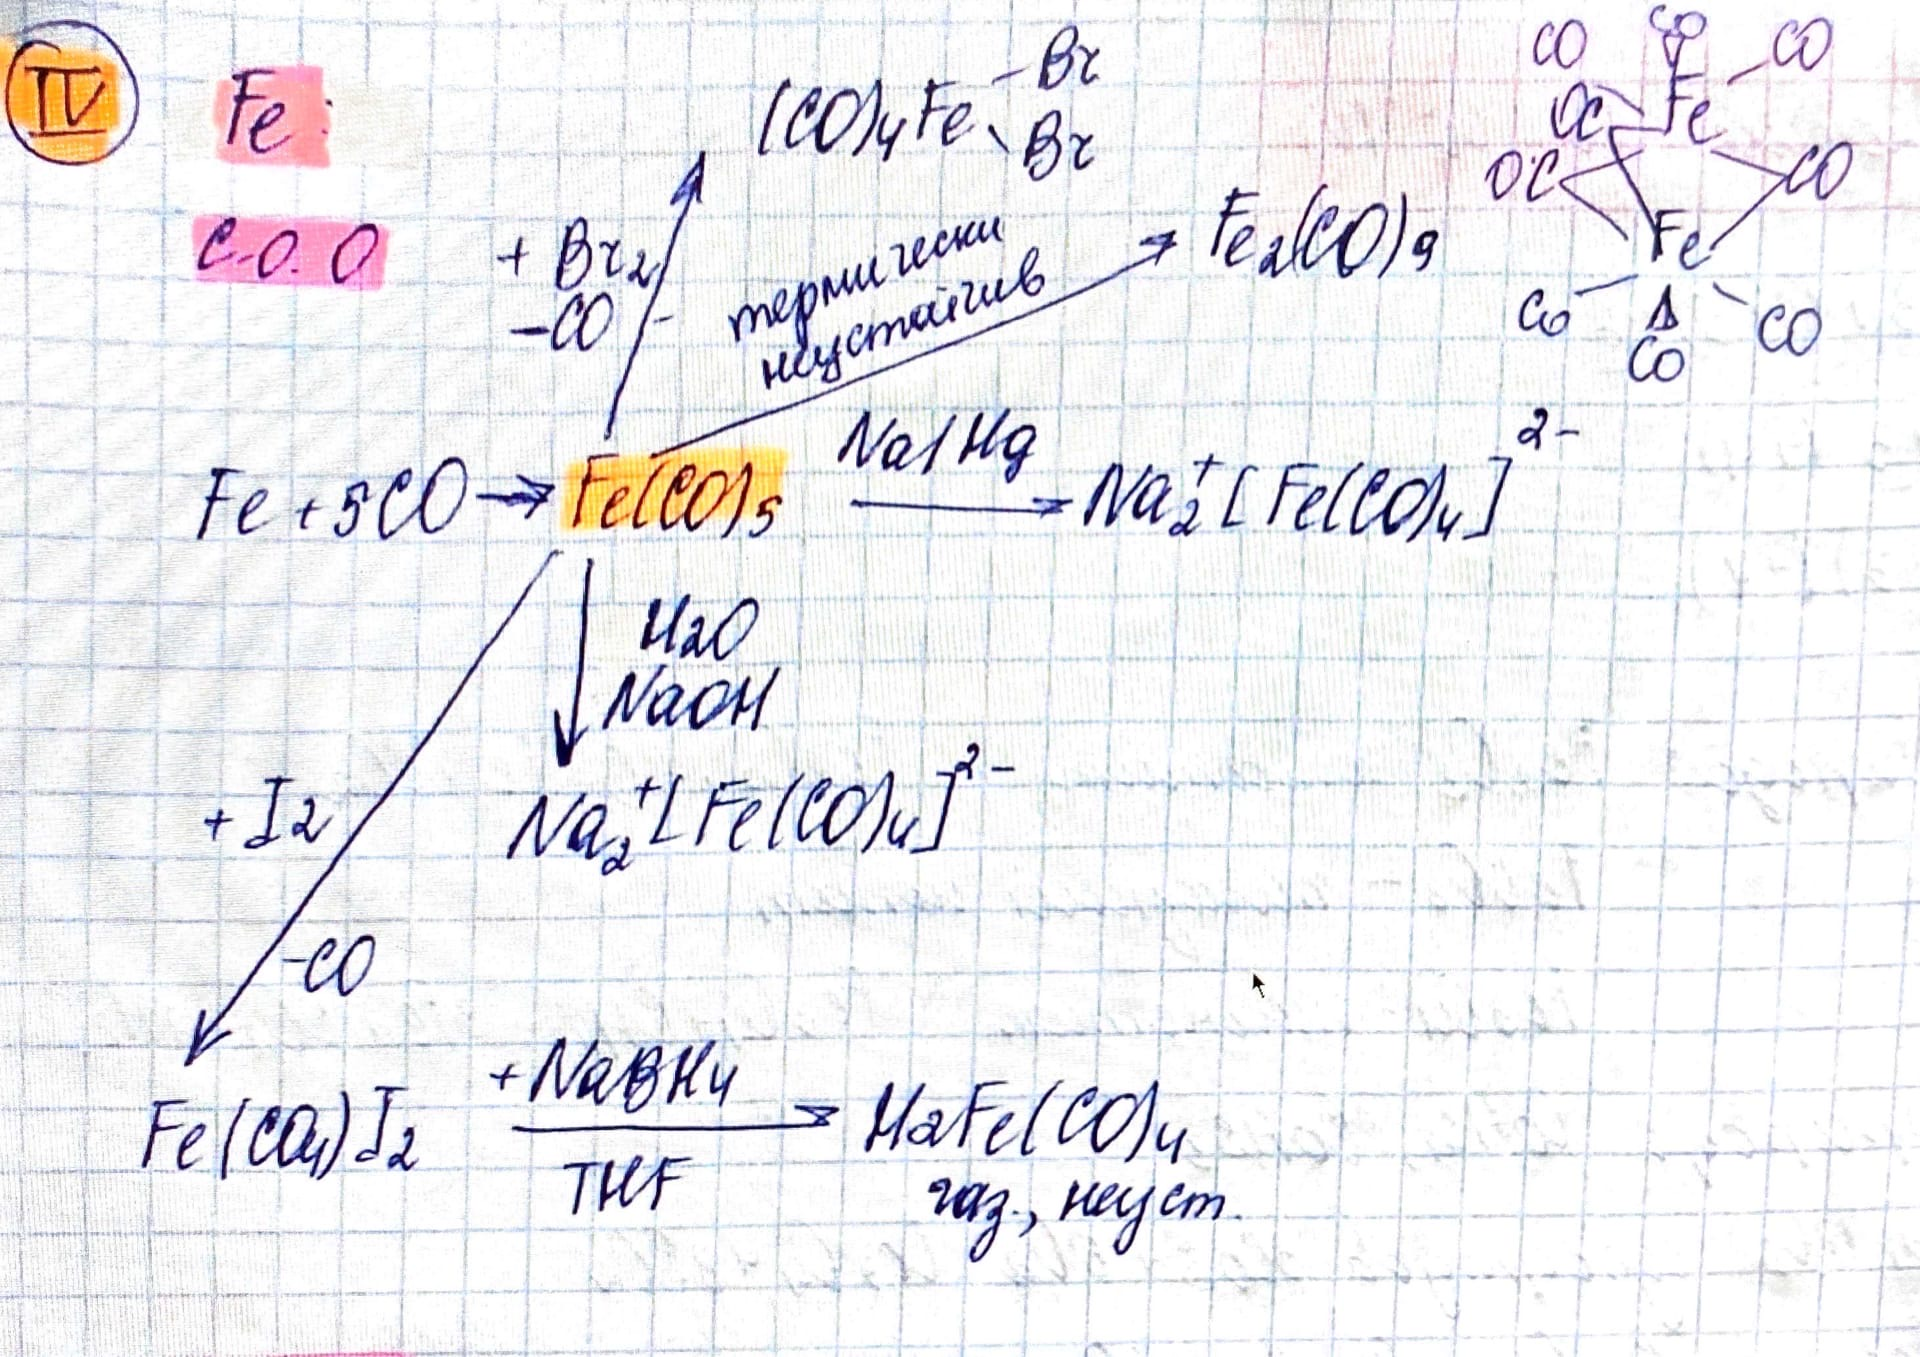
\includegraphics[scale=0.25]{ww1}}
\end{figure}
\textbf{Степень окисления $+2$}, ($d^6$)\\
\ul{Координационное число $6$}, высокоспиновые комплексы
\begin{align*}
&\left[Fe(H_2O)_6 \right]^{2-} \text{устойчивы аквакомплексы} \\
&FeCl_2 + 6 NH_3 = \left[Fe(NH_3)_6 \right]Cl_2 \\
&FeSO_4 + (NH_4)_2SO_4 = (NH_4)_2\left[Fe(SO_4)_2 \right] \cdot 6 H_2O \text{ (соль Мора)}
\end{align*}
Низкоспиновые комплексы с лигандами сильного поля: 
\[
\left[Fe(CN)_6 \right]^{4-}, \left[Fe(bpy)_3 \right]^{2+}, \left[Fe(phen)_3 \right]^{2+}, \left[Fe(en)_3 \right]^{2+}
\]
\ul{Координационное число $4$} \\
Тетраэдрические комплексы неустойчивы: $ \left[FeCl_4\right]^{2-}, \left[Fe(SCN)_4 \right]^{2-}$ \\
\ul{Координационное число $2$} \\
Объемные амидные лиганды: $\left[ Fe\{ N (SiMePh_2)_2 \}_2 \right]$ \\ \\
\textbf{Степень окисления $+3$}, ($d^5$)\\
Аммиакаты неустойчивы:
\[
FeBr_3 + 6NH_3 = \left[Fe(NH_3)_6\right]Br_3 = (H_2O) = \left[Fe(H_2O)_6\right]Br_3  
\]
Устойчивые с $\pi$-лигандами и хелатные:
\[
\text{высокоспиновые:} \left[Fe(H_2O)_6\right]^{3+}, \left[FeF_6\right]^{3-}, \left[Fe(ox)_3\right]^{3-}, \left[Fe(acac)_3\right] 
\]
\[
\text{низкоспиновые:} \left[Fe(CN)_6\right]^{3-}, \left[Fe(bpy)_3\right]^{3+}
\]
\ul{Координационное число $7$} \\
\[
\left[Fe(edba)(H_2O)\right]^{-}
\]
\ul{Координационное число $2$} \\
\[
\left[Fe(N(TMS)_2)_3\right] \text{ стабилизация амидными L}
\]
\textbf{Степень окисления $+4$} \\
$K_4FeO_4$ - тетраэдр, $d^4$, эффект Яна-Теллера \\
$12 KO_2 + Fe_3O_4 = 3K_4FeO_4 + 8 O_2$ - неустойчив в растворе, диспропорционирует \\
$FeF_2 + 2 CsF + XeF_2 = Cs_2\left[FeF_6 \right] + Xe$	\\ 
\textbf{Степень окисления $+5$} \\
$K_3FeO_4$ - тетраэдр \\
\textbf{Степень окисления $+6$} \\
Стабильность только в щелочном растворе:
\begin{align*}
2 Fe(OH)_3 + 10 KOH + 3 Br_2 &= 2K_2FeO_4 + 6KBr + 8H_2O \\
2K_2FeO_4 + 10H_2SO_4 &= 2Fe_2(SO_4)_3 + 3O_2 + 4K_2SO_4 + 10H_2O
\end{align*}
$FeO_4^{2-}$ - тетраэдр, парамагнитный \\ \\
$Co$: \\ \\
\textbf{Степень окисления $0$} \\
\[
2Co + 8CO = Co_2(CO)_8
\]
В двух формах:
\begin{figure} [H]
	\centering {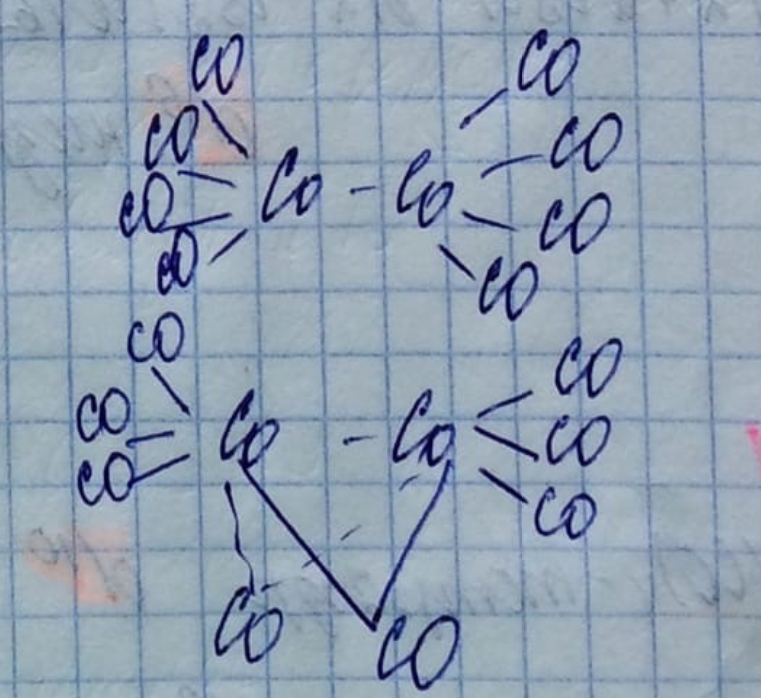
\includegraphics[scale=0.7]{ww2}}
\end{figure}
Образование мостиковой структуры более выгодно из-за размера ионов и участия $d$-орбитали.
\[
Co + 4CO + \frac12 H =   \left[Co(CO)_4 H \right] \text{ - сильная кислота}
\]
$Co_4(CO)_{12}$ - тетраэдрический кластер \\
\textbf{Степень окисления $+1$} \\
$\left[Co(PMe_3)_4\right]^+$ - тетраэдр \\
\textbf{Степень окисления $+2$}, ($d^7$)\\
нет предпочтительной конфигурации \\
\ul{Координационное число $2$} \\
Линейное строение $\left[ Co\{ N (SiMe_3) \}_2 \right]$ \\
\ul{Координационное число $3$} \\
Треугольное: $\left[ Co\{ N (SiMe_3) \}_2 (pph_3)\right], \left[ Co\{ N (SiMe_3)_2 \}_3 \right] $    \\
\ul{Координационное число $4$} \\
Тетраэдр: $\left[Co(Cl)_4 \right]^{2-}, \left[Co(OH)_4 \right]^{2-}  $ \\ 
\ul{Координационное число $5$} \\
Пирамида: $\left[Co(CN)_5 \right]^{3-}$   \\
\ul{Координационное число $6$} \\
Октаэдр: $\left[Co(H_2O)_6 \right]^{2+}$    \\
\ul{Координационное число $7,8$} \\
С краун-эфирами \\
\textbf{Степень окисления $+3$}, ($d^6$)\\
Устойчивы низкоспиновые комплексы $Co$ с $L$ сильного поля (кроме $\left[CoF_6 \right]^{3-}$) \\
Аквакомплекс $\left[Co(H_2O)_6 \right]^{3+}$ \\ \\
Аммиакаты с различным составом, инертны:
\[
\left[Co(NH_3)_6 \right]Cl_3, \quad \left[CoCl_2(NH_3)_4 \right]Cl, \quad \left[CoCl_3(NH_3)_3 \right]
\]
\textbf{Степень окисления $+4$}, ($d^5$)\\ 
Низкоспиновый:
\[
CoCl_2 + 2CsCl + 3 F_2 = Cs_2\left[CoF_6 \right] + 2Cl_2
\] \\ 
$Ni$: \\ \\
\textbf{Степень окисления $0$}, ($d^10$)\\
$Ni(CO)_4$ - тетраэдр \\
\textbf{Степень окисления $+1$}\\
Цианиды:
\[
K_2\left[Ni^{+2}(CN)_4 \right] = Na/Hg = K_4\left[Ni^{+1}(CN)_6 \right] = K/NH_3\text{(ж)} = K_4\left[Ni^{0}(CN)_4 \right]
\]
\textbf{Степень окисления $+2$}\\
\ul{Координационное число $4$} \\
$NiBr_2 + 2KBr = K_2\left[NiBr_4 \right]$ - устойчив, тетраэдр \\
Тетраэдры только с $L$ слабого поля \\
Квадратные с $L$ сильного поля: \\
$NiCl_2 + 4 KCN = 2 KCl + K_2\left[Ni(CN)_4 \right]$ \\
\ul{Координационное число $6$} \\
$\left[Ni(H_2O)_6 \right]^{2+}, \quad \left[Ni(NH_3)_6 \right]^{2+}, \quad \left[Ni(bpy)_3 \right]^{2+}$, олигомер $\left[Ni(acac)_2 \right]$ \\
\textbf{Степень окисления $+3$}, ($d^7$)\\
Относительно устойчивы фторокомплексы, сильные окислители, стабилизация $\sigma$ $\pi$-донорными $L$. \\
$ \left[NiBr_3(PEt_3)_2 \right] $ - низкоспиновый \\
$ \left[Ni_3(CH_3COO)_6 \right]^{3-} $ \\
\textbf{Степень окисления $+4$}, ($d^5$)\\
Стабилизация в гетерополисоединениях $(NH_4)\left[NiMo_9O_{32}\right]$ \\
$\left[NiF_6\right]^{2-}, \quad \left[NiIO_6\right]$ - окислители

